\documentclass[12pt,a4paper]{article}
\usepackage[utf8]{inputenc}
\usepackage[T1]{fontenc}
\usepackage{enumitem}
\usepackage{amsmath, amssymb}
\usepackage{graphicx}
\usepackage{hyperref}
\usepackage{comment}
\usepackage{tikz}
\usetikzlibrary{shapes, positioning, arrows.meta}


\usepackage[ruled,vlined,linesnumbered]{algorithm2e}
\SetKwInput{KwData}{Input}
\SetKwInput{KwResult}{Output}
\SetKw{KwTo}{to}
\SetKw{KwBy}{by}
\SetKw{KwRet}{return}

\usepackage{geometry}
\geometry{margin=2.5cm}

\title{\textbf{RulEvolution (Rul3volution): an evolutionary framework for rule-based learning}}
\author{Alia Rosario}
\date{}

\begin{document}
\sloppy

\maketitle

\begin{abstract}
This paper introduces a learning paradigm named \textit{RulEvolution} (or \textit{Rul3volution}), based on the application of logical rules modulated by dynamically varying weights that are updated through a learning algorithm. 
In contrast with deep neural models — extremely versatile and high-performing yet characterized by enormous complexity and limited transparency — the proposed model deliberately forgoes comparable performance in favor of stability, interpretability, and computational simplicity. 
A formal framework is introduced, built upon three fundamental concepts — rules, evolution, and stability — and a simple application to the \textit{TicTacToe} game is presented to demonstrate its feasibility and scalability. 
The system is also framed within the broader context of lifelong learning and \textit{Connectionless AI}, with a brief comparison to studies on \textit{Cognidynamics}.
\end{abstract}


\textbf{Keywords:} Rule-based learning, Evolutionary systems, Connectionless AI, Adaptive rules, Fuzzy logic, Explainable AI, Logic rules as semantic labels, Parallel computing.


\section{Introduction}
The act of addressing a problem involves understanding whether it can be entirely described through parameters and rules defined “\textit{a priori}”, or whether it contains elements that can only be identified “\textit{a posteriori}”.  
Classical algorithms assume that a problem is fully defined \textit{a priori}: the parameters are known or constrained by predictable rules.  
In such cases, the search for deterministic rules enables an effective algorithmic solution.  

However, the theory of computation has shown that not all well-formulated problems admit an algorithmic solution: some are undecidable or incomplete.  
When a deterministic solution is not available, heuristic or approximate methods are employed.  

There are also problems in which not all data or structures can be known in advance.  
For instance, the interpretation of natural language shows that a specific semantic content can be expressed in many different linguistic forms, making the definition of exhaustive rules impractical.  
In such contexts, the idea has emerged of creating tools capable of autonomously learning problem-solving strategies.  
The ability to learn is a powerful and versatile means of problem solving; even in the biological world, the large-scale adoption of this mechanism is evident.


\subsection{Learning and complex systems}
Machine learning systems capable of addressing complex issues have been successfully implemented by adopting \textit{Deep Neural Networks} (DNN) trained through the \textit{backpropagation} method. 
The achievements already reached by such neural networks are astonishing and are transforming the world, revealing further and promising developments ahead. 

We will not attempt to describe the highly sophisticated architectures of the latest neural networks; it is sufficient to note that the number of parameters involved in their design and configuration can exceed values on the order of $10^{12}$. 
These are systems that can only be described through statistical models and certainly belong to the class of what, in Physics, are called \textit{"Complex Systems"}.

\subsection{Limits of deep neural networks}

\paragraph{A) Computational problem.} 
The training and operation of deep neural networks require extremely powerful computing infrastructures (GPU, TPU, and dedicated clusters), entailing significant energy and environmental costs.

\paragraph{B) Training problem.} 
A massive amount of labeled and structured data is required to ensure satisfactory performance. 
The collection, management, and validation of such data represent an ongoing challenge.

\paragraph{C) Reliability problem.} 
As complex systems, neural networks exhibit emergent behaviors that can sometimes prove entirely unpredictable or even erroneous. 
Such instabilities make it difficult to explain and certify the reliability of the produced results.

The issues listed above motivate the search for alternative paradigms that are more stable, transparent, and understandable.


\section{The RulEvolution Concept}
The \textit{RulEvolution} paradigm proposed in this paper stems from the attempt to combine the classical algorithmic approach with the flexibility of machine learning. 
It is based on the idea that rules can be adapted over time through the assignment and evolution of associated weights, which progressively modulate their influence according to the experience acquired. 

The name itself — \textit{RulEvolution} or \textit{Rul3volution} — is meant to recall three key concepts:
\begin{enumerate}
\item \textbf{Rule}: every decision of the system derives from an explicit set of formally defined rules.
\item \textbf{Evolution}: the weights associated with the rules change over time as a function of experience, allowing a progressive adaptation of the system’s behavior.
\item \textbf{Stability}: this third concept is represented by the number \textit{3} in the name, which graphically replaces the letter \textit{E} and, at the same time, reverses the assonance with the word “Revolution”, emphasizing that the system preserves coherence and predictability, avoiding chaotic behavior.
\end{enumerate}

\subsection{How a RulEvolution agent operates}
The system acts by following a decision graph or, in particularly structured cases, a decision tree.  
At each branching of the graph, behavioral rules $r_i$ operate collectively as a logical driver that guides the system’s action along one of the possible paths.  
The rules suggest certain branches by assigning them weights\footnote{A rule, in principle, may suggest more than one path. In many decision processes, some choices are discarded while others are accepted. To give a trivial example, if the rule requires selecting a multiple of 2 and the possible branches are 3, 4, 5, and 6, it will discard 3 and 5 while positively evaluating 4 and 6, placing them on the same level.}.  
The sum of these weights measures the confidence assigned to each branch, and the decision-making process continues along a single branch, chosen according to two main criteria:

\begin{itemize}
    \item \textit{\textbf{Best-choice criterion} — deterministic selection}: the branch with the highest confidence estimate is chosen; if multiple branches receive the same confidence score, the system adopts a predefined selection criterion (such as for example a random choice).
    
    \item \textit{\textbf{Reflective-Exploration criterion} — probabilistic selection}: the system may select any branch under consideration, but the probability of choosing a given branch is proportional to the confidence score assigned to it.  
    In this way, a stochastic component is introduced that, in principle, allows the exploration of the entire decision tree; however, such randomness is strongly mitigated by the evaluation provided by the system’s logical rules \footnote{In some contexts, a minimum evaluation threshold can be introduced to exclude branches with very low scores, in order to limit the exploration of weakly promising paths.}.  
    Thus, the system maintains a balance between logical coherence and exploratory capability — a characteristic often desirable in an adaptive agent.
\end{itemize}

\subsection{Responses to twin inputs}
We will later address the learning aspects of the automatic system just described; for now, let us assume that the decision graph through which it operates does not evolve over time.  
If we provide this system with two \textit{twin inputs} (i.e., two identical inputs in sequence), its behavior will depend on the selection criterion adopted:
\begin{itemize}
\item with the \textit{best-choice criterion}, the agent will produce identical or substantially equivalent responses;
\item with the \textit{Reflective-Exploration criterion}, especially in the presence of articulated decision trees, it is more likely to obtain different outputs, though still coherent and reasonable.
\end{itemize}
The choice between the two approaches depends on the nature of the problem: the first privileges stability and determinism, while the second favors flexibility, unpredictability, and, in some cases, behaviors that may recall very elementary forms of “creativity.”

\subsection{Weight updating and learning threshold}
The weight-updating mechanism constitutes the core of the \textit{RulEvolution} system’s adaptability and defines the dynamics of its ability to learn from experience.

After each computation, the final choice made by the decision graph is evaluated through a \textit{cost function}.  
The cost function can take different forms depending on the type of problem addressed and the design choices adopted.  
By way of example, two significant types of cost functions are described below, without any claim to exhaustiveness:

\begin{enumerate}[label=\alph*)]
\item \textbf{Example-based cost functions.}  
   These are used in supervised learning cases, where the system is provided with examples consisting of pairs of input and correct output.  
   The system evaluates the \textit{distance} between the computed result and the expected one and updates its parameters to minimize this \textit{distance}.  
   Such learning requires a sufficiently large and representative training dataset.

\item \textbf{Expected-value cost functions.}  
   These can be employed when the objective to be achieved is objectively definable, for instance: winning a game or locating an object in a search process.  
   This approach enables forms of self-learning, since the system can autonomously evaluate the “goodness” of the outcome and assign an appropriate merit score to the achieved performance.
\end{enumerate}

After each experience — that is, after each action for which the corresponding \textit{cost function} can be computed — the system updates the weights of the logical rules to minimize that cost.  
A general criterion to guide the adjustment of weights consists in keeping track of the rules applied along the path of the decision graph that led to the obtained solution.  
If the solution is deemed valid, the weights of the involved rules are increased; if the solution is judged invalid, they are decreased.  
A neutral case may also be considered, in which the weights remain unchanged.

In symbolic form, the rule for weight evolution can be expressed as:
\[
w_i(t+1) = w_i(t) \pm \tau,
\]
where $\tau$ represents the \textit{learning rate}, and the positive or negative sign is chosen according to the quality of the obtained result.

However, applying this technique directly to every single case can produce “nervous” learning — that is, learning that is overly sensitive to local variations and unable to capture the desired overall trend of the system.  
Such unstable behavior should be avoided, as it risks compromising the coherence of adaptation.

\subsection{Introducing a counter}  
To mitigate such instabilities, an experience-accumulation mechanism based on a counter $c$ can be introduced.  
Each time a solution is deemed a valid or invalid consequence of a given rule, the system does not immediately modify the corresponding weight $w_i$, but instead increments or decrements a counter $c_i$.  
Only when $c_i$ exceeds a given positive threshold $+\sigma$ or negative threshold $-\sigma$ is the weight $w_i$ actually updated.  
This mechanism makes the variation of the weights depend on a set of events rather than on a single episode, thereby making learning more stable and coherent over time.

\bigskip

\begin{algorithm}[H]
\caption{Weight updating with threshold and counter}

\medskip
\KwData{set of active rules $\{r_i\}$ in the decision path}
\KwResult{updated weights $\{w_i\}$}
\bigskip

\ForEach{rule $r_i$ used}{
    \eIf{the solution is valid}{
        $c_i \leftarrow c_i + 1$ \;
    }{
        $c_i \leftarrow c_i - 1$ \;
    }
    \If{$c_i \ge +\sigma$}{
        $w_i \leftarrow w_i + \tau$ \;
        $c_i \leftarrow 0$ \;
    }
    \If{$c_i \le -\sigma$}{
        $w_i \leftarrow w_i - \tau$ \;
        $c_i \leftarrow 0$ \;
    }
}
\end{algorithm}

\bigskip

$\tau$ represents the \textit{learning rate}, while $\sigma$ denotes the \textit{accumulation threshold} required for an effective weight update.  
In this way, the weight update becomes the result of a persistent trend rather than a single fluctuation, thus reinforcing the overall stability and coherence of the system.


\section{Connectionless AI and lifelong learning}
\textit{RulEvolution} systems are inspired by the principles of \textit{Connectionless AI}, aiming to develop intelligent behaviors even in the absence of large training datasets.

Since the behavior of a \textit{RulEvolution} system is always guided by the application of logical rules, it is capable of operating intelligently from the very beginning, progressively refining its performance throughout its operational life.

Drawing a parallel with biological systems, the basic structure formed by the decision graph and the logical rules it contains can be compared to the innate and instinctive component of a living being, whereas the continuous adaptation of rule weights recalls the learning and evolutionary processes typical of the natural world.  
As in biology, the system does not necessarily evolve toward an absolutely “better” form, but rather toward a “more suitable” one for the task to be accomplished, with the goal of optimizing its operational effectiveness.

In the context of lifelong learning and \textit{Connectionless AI}, it is appropriate to mention the studies of Professor \textit{Marco Gori} and the research group at the University of Siena, who developed the concepts of \textit{Cognidynamics}, \textit{Hamiltonian Learning}, and \textit{NARNIAN} systems (\textit{NAtuRe-iNspIred computAtional IntelligeNce agents}).

The approach pursued by this group is highly innovative and promising, and it differs deeply, both conceptually and methodologically, from the \textit{RulEvolution} paradigm.  
The operation of \textit{NARNIAN} systems is not based on the application of explicit logical rules embedded in a decision graph and applied to events that occur in a discrete temporal sequence.  
\textit{Cognidynamics} employs the methodologies and tools of Optimal Control and Automatic Systems Theory to design intelligent agents capable of continuous learning and operation in continuous time, described by a real parameter rather than a discrete one. {\footnote{For further details on \textit{NARNIAN} systems, see the bibliographic references and the website: \\ \url{https://sites.google.com/unisi.it/lot-spring-school/}}}


Although the \textit{Cognidynamics} paradigm is grounded on a different theoretical framework, the conceptual inspiration provided by these studies has undoubtedly been valuable in the preparation of this work.


\section{Degrees of Freedom, Number of Experiences, and History: key parameters for a learning system}

The effectiveness of a generic learning system depends on several factors.  
This section focuses on three characteristics, each expressible by an integer number, that are significant in describing the system’s ability to adapt, store information, and stabilize its behavior over time.  
These three parameters have general validity; here, they are used to compare deep neural networks (DNN) and \textit{RulEvolution} systems.

\subsection{Degrees of freedom ($f$)}
Let $f$ (\textit{freedom}) denote the number of degrees of freedom of a learning system.  
$f$ is the dimensionality of the system’s configuration space, meaning that the global behavior is assumed to be determined by $f$ parameters governing its dynamics.  
Intuitively, it is reasonable to assume that, all other things being equal, the greater the number of degrees of freedom, the broader the class of problems the system can address.  

In the case of deep neural networks (DNN), $f$ can reach values on the order of $10^{12}$, providing extremely high flexibility but also resulting in enormous computational complexity and interpretability challenges.  
In \textit{RulEvolution} systems, by contrast, the number of parameters drops dramatically: even a complex system rarely exceeds 100 degrees of freedom, and in many cases, it uses fewer than 10.  
Such a reduced configuration space limits overall flexibility but offers significant advantages in terms of computational cost, transparency, control, and stability.  

\subsection{Number of experiences ($e$)}
A second fundamental parameter is the number of experiences, denoted by $e$, representing the amount of examples or interactions required for effective training.  
A system that requires a very large number of examples entails a higher training cost but also a greater learning and fine-tuning capability.  
However, training is never a definitively completed process: additional examples can always refine the system’s behavior.  

In practical applications, training can be considered complete when:
\begin{enumerate}[label=\alph*)]
    \item the system successfully passes numerous and diversified performance tests;
    \item the learning parameters converge, meaning that the addition of new examples no longer significantly alters the learning parameters.
\end{enumerate}

Deep neural networks require extremely large training datasets to converge, whereas \textit{RulEvolution} systems can complete the learning phase with a much smaller number of examples, thereby reducing both time and computational costs.

\subsection{History ($h$)}
The third parameter, denoted by $h$, represents the \textit{history} of the system, that is, its memory of past experiences.  
$h$ indicates the number of experiences the system can retain and process collectively in order to update its behavior. Let us examine the importance of this parameter.

When training occurs by processing experiences one at a time, the learning coordinates may be strongly influenced by anomalous values (\textit{outliers}), which can shift the system’s state into suboptimal regions of the configuration space.  
Escaping from such regions may be difficult and require a long period of retraining.

A useful analogy to understand this phenomenon can be found in human cognitive processes: a deeply traumatic experience can be interpreted as an “emotional outlier” that profoundly alters an individual’s learned behavior, shifting it into pathological regions analogous to suboptimal states.  
To mitigate such effects, training data analysis should not be limited to a single experience but extended to a group of experiences.  
The analysis of a set of experiences also allows statistical quantities such as mean, variance, maxima and minima, or evolutionary trends to be considered, all of which can provide valuable guidance to the learning process.  
A higher value of $h$ corresponds to a broader memory and, consequently, to potentially more stable, robust, and effective learning.

It is not always possible to estimate the numerical value of $h$ precisely; often it can only be defined approximately or empirically.  

In deep neural networks, the historical evaluation of training data occurs indirectly: since there is an enormous number of parameters, they are not all heavily and simultaneously affected by a single observation.  
The network thus implicitly stores the history of the inserted data through its complexity, effectively using a form of “distributed memory.”

In \textit{RulEvolution} systems, on the other hand, historical memory is managed explicitly: the variation of weights occurs only when the cumulative sum of experience evaluations reaches a threshold value $\sigma$.  
The number $h$ (history) and the threshold $\sigma$ do not coincide but are correlated quantities: the higher the threshold, the greater the number of experiences evaluated before modifying the corresponding parameter.  

For all machine learning systems — not only those considered in this paper — it will be useful to develop increasingly effective techniques to evaluate and leverage the “history” of training data.  
This represents an important direction for future research in adaptive systems.


\section{Comparison between deep neural network systems with backpropagation and RulEvolution systems}

Deep Neural Networks (DNN) and \textit{RulEvolution} systems represent two conceptually and architecturally different learning paradigms.  
The comparison between these models highlights advantages and limitations in several complementary domains, which can be summarized as follows:

\begin{itemize}
    \item \textbf{Degrees of freedom.}  
    DNNs have a number of parameters on the order of $10^{12}$, a scale that grants them extraordinary flexibility and the ability to adapt to a wide range of problems.  
    The power and flexibility of neural networks derive not only from the vast number of parameters but also from their ingenious tuning method, known as “backpropagation.”  
    However, such complexity entails high computational costs and significant difficulties in interpreting their internal behavior.  
    \textit{RulEvolution} systems, on the other hand, operate with a much smaller number of parameters (often fewer than 100), drastically reducing the complexity of the configuration space and making the system’s evolution far more controllable.

    \item \textbf{Architecture and specialization.}  
    DNNs are general-purpose models, capable of adapting to different domains through the automatic training of weights; a single model can address very diverse tasks, provided that an adequate set of examples is available.  
    \textit{RulEvolution} systems, by contrast, are designed from the outset for a specific application domain: the rules that compose them are defined \textit{a priori} and subsequently modulated through adaptive weights.  
    Learning does not construct the system’s behavior but progressively refines its coherence and efficiency.  
    This approach requires greater initial design effort but ensures specialization, transparency, and stability.

    \item \textbf{Computational cost.}  
    The large number of parameters in DNNs necessitates dedicated hardware infrastructures (GPU, TPU, and computing clusters), resulting in considerable energy and environmental costs.  
    \textit{RulEvolution} systems, instead, operate with modest computational resources, making them suitable even for embedded or distributed contexts, while still maintaining the capability of progressive learning.

    \item \textbf{Interpretability and traceability.}  
    In DNNs, parameters do not have a direct semantic meaning, and global behavior emerges from complex statistical interactions, that are often difficult to interpret.  

    In a \textit{RulEvolution} system, each weight is explicitly associated with a logical rule, which in fact serves as a \textit{\textbf{semantic label}} for the learning parameter.  
    This allows the immediate identification of the contribution of each decision component.  
    Debugging is also easier thanks to the traceability of the causes behind anomalous behaviors.

An additional advantage of \textit{RulEvolution} systems concerns their maintenance and evolution.  
During revision, it may be observed that the weight of a rule grows excessively, in a manner not anticipated during the initial design.  
This typically occurs when a behavioral rule is activated too frequently because it applies to an overly broad family of contexts.  
In such cases, it is advisable to consider whether the rule in question should be further specialized—perhaps split into two or more subrules—to make the system’s action more specific.   

    \item \textbf{Stability and emergent behaviors.}  
    Due to their nonlinear and dynamic structure and the very high number of parameters, deep neural networks belong to the class of systems that, in Physics, are referred to as \textbf{“Complex Systems.”}  
    As such, they exhibit both desirable emergent behaviors and occasional, hardly predictable instabilities that can compromise the reliability of their results.  

    A \textit{RulEvolution} system, based on explicit rules and controlled updates, can ensure greater predictability and consistency over time.

    \item \textbf{Overfitting.}  
    Another limitation of DNNs is the phenomenon of \textit{overfitting}, that is, the tendency of the model to excessively memorize training data, losing its ability to generalize to new data.  
    This effect arises from the high number of degrees of freedom and the vastness of the search space.  


    \textit{RulEvolution} systems, thanks to their more constrained structure and reduced number of parameters, are inherently less prone to overfitting, while still maintaining a good level of adaptability.  
	Moreover, the clear correspondence between weights and rules makes it easy to detect potential over-specializations and correct them during the debugging phase, by directly modifying the formulation of the rules themselves.

\end{itemize}

In summary, DNNs represent general-purpose models with high predictive power but limited controllability, whereas \textit{RulEvolution} systems offer a balanced compromise between adaptive capability, computational efficiency, and interpretive transparency.  
Both paradigms share the same ultimate goal—learning from experience—but they pursue it through profoundly different strategies: the former relying on the mass of data, the latter on the clarity of rules.


\section{RulEvolution and possible Fuzzy extensions}

A potential development of the \textit{RulEvolution} paradigm draws inspiration from Fuzzy Logic, whose fundamental notions were introduced by Zadeh (1965).

A \textit{RulEvolution} system could be designed to employ both classical Boolean rules of the \textit{crisp} type and \textit{Fuzzy} rules, capable of handling uncertainty and gradual transitions in a more transparent and flexible way.  
Such an approach would make it possible to broaden the range of application domains while maintaining interpretability and stability.  

There are already numerous areas in which Fuzzy Logic has been successfully applied, for example:

\begin{itemize}
    \item \textbf{Automatic control}: regulation of temperature, speed, and complex industrial processes.
    \item \textbf{Classification systems and differential diagnostics}: decision support in the presence of uncertain or incomplete data.
    \item \textbf{Evaluation and assessment systems}: qualitative or semi-quantitative analysis tools based on graded judgments.
    \item \textbf{Computer vision and pattern recognition}: identification of shapes or objects under conditions of uncertainty or perceptual ambiguity.
\end{itemize}

In these areas, the integration of Fuzzy Logic within a \textit{RulEvolution} system has strong potential to prove fruitful, enhancing the system’s ability to adapt to real-world contexts without sacrificing interpretive transparency.


\section{Application of RulEvolution to TicTacToe}

As a conceptual proof, a \textit{RulEvolution} system was developed for the \textit{TicTacToe} game.

The goal is not to create an optimal player (many other validated techniques already exist to build an automatic TicTacToe player), but rather to experimentally verify the proposed paradigm by testing the dynamics of learning and weight updating in a controlled and easily analyzable environment.

The source code of the system was written in \texttt{C++} and is available at the following link:\\
\href{https://github.com/r-alia-sicily/rulEvolution-tictactoe/tree/main}
{\texttt{https://github.com/r-alia-sicily/rulEvolution-tictactoe/tree/main}} \textbf{(GitHub Repository)},\\
where possible future versions — including those in other programming languages — as well as the \LaTeX{} source code of this paper will be published.

\subsection{Motivation for choosing the TicTacToe game}

\textit{TicTacToe} is a game of extreme simplicity, characterized by a limited number of possible states and by clear, finite rules.

A complete match may require between three and five moves per player,\footnote{Counting the moves of a single player: five moves are reached if the player starts first and the board is completely filled.}
making it an ideal initial testing ground for observing the effects of logical rules, weight dynamics, and learning stability.

Naturally, for more complex applications, the \textit{RulEvolution} paradigm will need to be tested in more articulated, challenging, and realistic domains.

\subsection{General system structure}

The nine cells of the board are numbered from left to right and top to bottom, from 0 to 8, as illustrated in Figure~\ref{fig:tictactoe-grid}.  

\begin{figure}[h!]
\centering
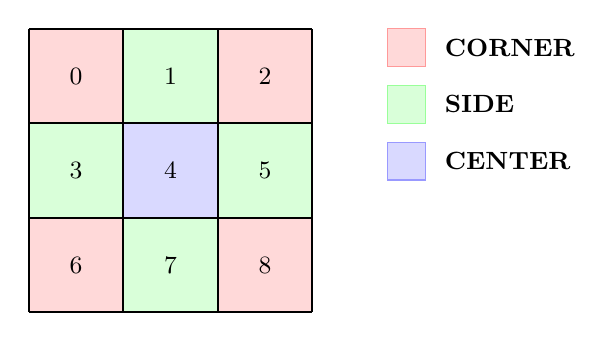
\begin{tikzpicture}[scale=1.2, every node/.style={font=\small}]
% Fills before the grid
\fill[blue!15] (1,1) rectangle (2,2); % CENTER
\fill[red!15] (0,2) rectangle (1,3);  % CORNER 0
\fill[red!15] (2,2) rectangle (3,3);  % CORNER 2
\fill[red!15] (0,0) rectangle (1,1);  % CORNER 6
\fill[red!15] (2,0) rectangle (3,1);  % CORNER 8
\fill[green!15] (1,2) rectangle (2,3); % SIDE 1
\fill[green!15] (0,1) rectangle (1,2); % SIDE 3
\fill[green!15] (2,1) rectangle (3,2); % SIDE 5
\fill[green!15] (1,0) rectangle (2,1); % SIDE 7

% Main grid
\draw[thick] (0,0) grid (3,3);

% Cell numbering
\node at (0.5,2.5) {0};
\node at (1.5,2.5) {1};
\node at (2.5,2.5) {2};
\node at (0.5,1.5) {3};
\node at (1.5,1.5) {4};
\node at (2.5,1.5) {5};
\node at (0.5,0.5) {6};
\node at (1.5,0.5) {7};
\node at (2.5,0.5) {8};

% Legend
\begin{scope}[shift={(3.8,1.5)}]
\draw[red!40,fill=red!15] (0,1.1) rectangle +(0.4,0.4);
\node[right] at (0.5,1.3) {\textbf{CORNER}};
\draw[green!40,fill=green!15] (0,0.5) rectangle +(0.4,0.4);
\node[right] at (0.5,0.7) {\textbf{SIDE}};
\draw[blue!40,fill=blue!15] (0,-0.1) rectangle +(0.4,0.4);
\node[right] at (0.5,0.1) {\textbf{CENTER}};
\end{scope}
\end{tikzpicture}
\caption{Strategic cell categories in the \textit{TicTacToe} game.}
\label{fig:tictactoe-grid}
\end{figure}

\subsection{Types of players}

The system allows for three types of players:
\begin{itemize}
    \item \textbf{Human}: a human player who enters moves from the keyboard;
    \item \textbf{Stochastic}: a player who chooses moves randomly;
    \item \textbf{RulEvolution}: a player who makes decisions based on a set of weighted, evolutionary, and adaptive logical rules.
\end{itemize}

\subsection{Right to the first move}
Which player — X or O — has the right to the first move is determined randomly at the beginning of each game.

\subsection{Overview of the decision logic of the RulEvolution player}

At each turn, the system examines the free cells of the board and assigns each a score.  
The move to play is selected according to the overall evaluation derived from the application of a set of logical rules.  
Each rule assigns a score to one or more cells, and during every turn, the system computes a total score for each cell by summing the contributions of the individual decision rules.

\subsection{Decision rules of the RulEvolution-TicTacToe system}

The rules that compose the \textit{RulEvolution-TicTacToe} system are divided into three main categories.

\paragraph{A) Strategic position gain rules}
\begin{itemize}
    \item \textbf{CENTER}: occupy the center of the board (cell 4).  
    The player occupying the center cell has the possibility of completing 4 potential winning lines, so the initial weight (i.e., before training) assigned to this cell should be proportional to the value $4$.
    \item \textbf{CORNER}: occupy a corner (cells 0, 2, 6, 8).  
    The player occupying a corner cell can complete 3 potential winning lines, so the initial weight (i.e., before training) assigned to these cells should be proportional to the value $3$.
    \item \textbf{SIDE}: occupy a side (cells 1, 3, 5, 7).  
    The player occupying a side cell can complete 2 potential winning lines, so the initial weight (i.e., before training) assigned to these cells should be proportional to the value $2$.
\end{itemize}

\paragraph{B) Tactical context rules}
\begin{itemize}
    \item \textbf{WIN}: if the player occupies two aligned cells and the third one is free, choose that cell to win.  
    The weight of the \textbf{WIN} rule is set very high (potentially infinite) and does not need to be modified by training — a “\textit{universally valid choice}.”
    \item \textbf{BLOCK}: if the opponent occupies two aligned cells and the third one is free, this rule aims to occupy it to prevent victory.  
    High weight, but lower than \textit{WIN}.
\end{itemize}

\paragraph{C) Rules for preparing victory}
\begin{itemize}
    \item \textbf{PREPARATION}: choose cells that, together with those already occupied, create one or more potentially winning configurations (occupy two aligned cells with a third currently free).  
    If a cell contributes to two possible future winning lines, it receives a double score.
\end{itemize}

\subsection{Move evaluation and selection}

The rules described above generate, at each turn, a set of scores for each free cell on the board.  
For each cell, the sum of the contributions provided by the various rules represents the degree of \textit{confidence} that the system assigns to occupying that specific position in the current turn.

If the system always chose the cell with the maximum score, its behavior would become predictable and devoid of strategic variability.  

To avoid such deterministic rigidity, a controlled stochastic criterion is adopted — a simplified version of the previously discussed \textit{\textbf{Reflective-Exploration criterion}}.

The cell to be occupied is selected with a probability proportional to the confidence score associated with each of them.

In this way, the move selection retains a random component — making the behavior unpredictable — while remaining guided by a coherent logic based on the system’s rules.

The algorithm responsible for selection constructs a continuous interval by arranging, as adjacent segments, the confidence values assigned to all available cells.  
A random number is then uniformly drawn within this interval;  
the cell corresponding to the subinterval in which the number falls is selected as the actual move.

In probabilistic terms, the selection is thus proportional to the width of the subinterval associated with each cell, ensuring that the most promising moves are more likely, while preserving a margin of exploration and behavioral diversity.

\subsection[Training mode and cost function for TicTacToe]
{Training mode \\ and cost function for TicTacToe}

Training is not always active; it is enabled only by user command and can occur only if at least one of the two players is of the \textit{RulEvolution} type.  
When two \textit{RulEvolution} players face each other, both undergo learning.

The cost function is based on the "\textbf{zero-sum}" nature of \textit{TicTacToe}: a game may end in a win, a loss, or a draw.  
The system records the rules applied during the match and the number of times each rule was activated.

At the end of the game:
\begin{itemize}
    \item in case of victory, the counters of the rules used are incremented;
    \item in case of defeat, they are decremented;
    \item in case of a draw, they remain unchanged.
\end{itemize}

This simple mechanism progressively strengthens effective rules and decreases the weight of less advantageous ones.


\section{Parallelization of the RulEvolution-TicTacToe system}

The initial version of the system was completely sequential.  
A parallel version was subsequently developed to evaluate the scalability of the paradigm.

\subsection{Parallel application of rules}

The rules contributing to move evaluation are independent of one another and can therefore be executed in parallel.  

Each rule, executed in parallel with the others, computes its own contribution to the score on the available cells, and the results are then summed at the output stage.


\subsection{Training through parallel games}

If the hardware resources allow, multiple games can be executed in parallel, properly synchronizing the rule counters shared among the processes.  
This approach accelerates the learning phase and demonstrates the intrinsic scalability of the \textit{RulEvolution} paradigm.

The \textit{RulEvolution-TicTacToe} system was parallelized to assess its suitability for parallel architectures.  
Although the gain in time and efficiency for such a simple game is minimal, the approach proves promising for more complex systems.  
This configuration makes it possible, in perspective, to perform distributed training of cooperating \textit{RulEvolution} agents even across heterogeneous clusters, paving the way for forms of collective and unsupervised learning.

\bigskip
The \textit{RulEvolution-TicTacToe} system serves as a conceptual laboratory for the study of learning based on evolutionary rules.  
Despite its simplicity, it demonstrates the feasibility of an alternative approach to neural models.


\section{Conclusions and future developments}
The \textit{RulEvolution} paradigm represents an attempt to reconcile the logical solidity of expert systems with the plasticity of machine learning.  
  
The reduction in the number of parameters, the clarity and interpretability of the rules, and the stability of the results constitute its main strengths.  
  
Future developments will focus on the fuzzy extension and on applications to more complex contexts, while maintaining as a fundamental objective the transparency and certifiability of the system’s behavior.

\section*{References}

\begin{itemize}

\item Gori, M. (2024). \textit{An Introduction to Cognidynamics}. arXiv:2408.13112v1.

\item Zadeh, L. A. (1965). \textit{Fuzzy Sets}. \textit{Information and Control}, 8(3), 338–353.

\item Kosko, B. (1992). \textit{Neural Networks and Fuzzy Systems: A Dynamical Systems Approach to Machine Intelligence}. Prentice Hall.

\item Russell, S. J., \& Norvig, P. (1995). \textit{Artificial Intelligence: A Modern Approach}. Prentice Hall.

\item Holland, J. H. (1975). \textit{Adaptation in Natural and Artificial Systems}. University of Michigan Press.

\item Rumelhart, D. E., Hinton, G. E., \& Williams, R. J. (1986). \textit{Learning Representations by Back-Propagating Errors}. \textit{Nature}, 323, 533–536.

\item Giorgi, R. (2023). \textit{Parallel Programming Fundamentals}. Course held at the University of Siena, Department of Information Engineering (PhD Course in Information Engineering and Science). \url{https://phdies.diism.unisi.it/corsi/corsi.php}

\item Giorgi, R. (2024). Faculty profile and research activities. University of Siena. \url{https://docenti.unisi.it/en/giorgi-1}

\item Larsson Träff, J. (2024). \textit{Lectures on Parallel Computing}. arXiv:2407.18795.

\item Gori, M., \& Melacci, S. (2017). \textit{Deep Learning: Lecture Notes}. University of Siena, Master’s Degree in Computer Engineering.

\item Schmidhuber, J. (1990). \textit{A Possibility for Implementing Curiosity and Boredom in Model-Building Neural Controllers}. In \textit{Proc. SAB '91}, MIT Press.

\item von Neumann, J. (1958). \textit{The Computer and the Brain}. Yale University Press.

\end{itemize}

\end{document}